\documentclass{beamer}
% Use DS9 global theme (includes pgfplots for visualization)
\usepackage{../../../shared/templates/ds9_theme}

% Title page configuration
\title[Variable Scope]{CS12 CH: Variable Scope}
\subtitle{Visibility, Lifetime, and Memory Management}
\author[Mr. Gullo]{Mr. Gullo}
\date[Dec 04]{December 04, 2025}

\begin{document}
\frame{\titlepage}

\begin{frame}
\frametitle{Learning Objectives}
By the end of this lesson, you will be able to:
\begin{itemize}
    \item \textbf{Define} variable scope and determine where a variable is accessible within a program.
    \pause
    \item \textbf{Distinguish} between Local and Global scope.
    \pause
    \item \textbf{Explain} the difference between Pass-by-Value (copy) and Pass-by-Reference (alias).
    \pause
    \item \textbf{Identify} variable shadowing and predict the output of nested scopes.
    \pause
    \item \textbf{Implement} functions using reference parameters to modify external variables.
\end{itemize}
\end{frame}

% ==========================================
% SECTION 1: BASIC SCOPE & LOCALITY
% ==========================================

\begin{frame}
\frametitle{What is Scope?}
\begin{block}{Definition}
\textbf{Scope} is the region of code where a specific variable is visible and accessible.
\end{block}

\pause
\vspace{1em}
\textbf{Key Rules:}
\begin{itemize}
    \item Variables declared inside a function are \textbf{local} to that function.
    \pause
    \item Other functions cannot ``see'' or access these variables.
    \pause
    \item Local variables are destroyed when the function ends.
\end{itemize}
\end{frame}

\begin{frame}
\frametitle{Concept Visualization: Scope Isolation}
\textbf{The Concept:}
Think of every function as a soundproof room.

\pause
\vspace{1em}
\begin{itemize}
    \item If you say a number inside \texttt{main()}, the function \texttt{display()} cannot hear it.
    \pause
    \item To share information, you must explicitly pass a note (parameter) through the door.
\end{itemize}

\pause
\vspace{1em}

\end{frame}

\begin{frame}
\frametitle{Visualizing Memory Isolation}
% Diagram representing separate memory scopes
\begin{center}
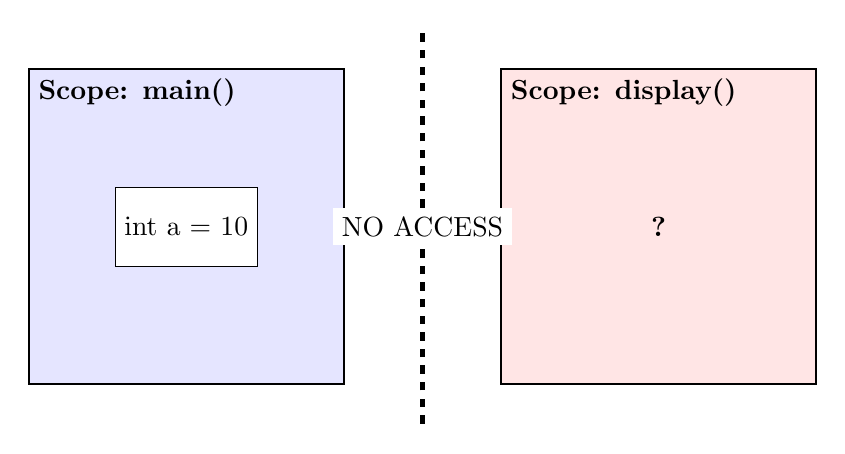
\begin{tikzpicture}
    % Main Scope
    \draw[fill=blue!10, thick] (0,0) rectangle (4,4);
    \node[anchor=north west] at (0,4) {\textbf{Scope: main()}};
    \node[draw, fill=white, minimum size=1cm] (A) at (2,2) {int a = 10};

    % Other Function Scope
    \draw[fill=red!10, thick] (6,0) rectangle (10,4);
    \node[anchor=north west] at (6,4) {\textbf{Scope: display()}};
    \node (B) at (8,2) {\textbf{?}};
    
    % Barrier
    \draw[ultra thick, dashed] (5,-0.5) -- (5,4.5);
    \node[fill=white] at (5,2) {NO ACCESS};

\end{tikzpicture}
\end{center}
\end{frame}

\begin{frame}[fragile]
\frametitle{The Wall of Scope}
Attempting to access a local variable from another function results in a compiler error.

\begin{minted}[fontsize=\small]{cpp}
void display() {
    // ERROR: 'a' lives in main, not here.
    cout << a << endl; 
}

int main() {
    int a = 10; // Local to main
    display();
    return 0;
}
\end{minted}
\end{frame}

% ==========================================
% SECTION 2: PASS BY VALUE
% ==========================================

\begin{frame}
\frametitle{Pass by Value (The Copy)}
\begin{itemize}
    \item By default, C++ passes variables by \textbf{value}.
    \pause
    \item This means the function receives a \textbf{copy} of the data.
    \pause
    \item Changes to the parameter inside the function \textbf{do not} affect the original variable.
\end{itemize}

\pause
\begin{block}{Analogy}
If you email a spreadsheet to a friend, and they change the numbers, your original file on your computer does not change. They only have a copy.
\end{block}
\end{frame}

\begin{frame}
\frametitle{Visualizing Pass by Value}
% Diagram showing variable copying
\begin{center}
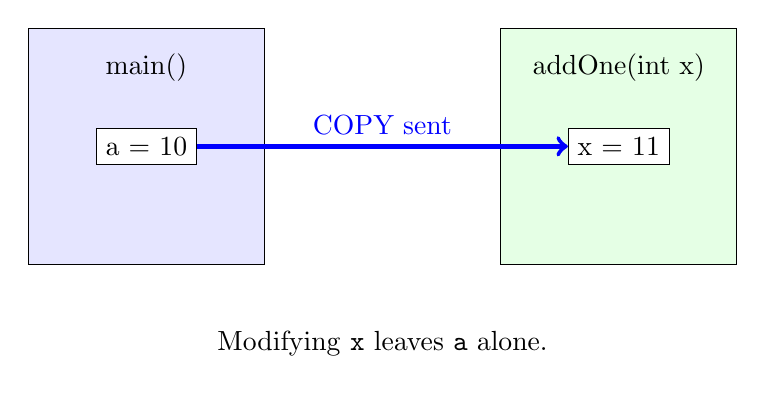
\begin{tikzpicture}
    % Main Scope
    \draw[fill=blue!10] (0,0) rectangle (3,3);
    \node at (1.5,2.5) {main()};
    \node[draw, fill=white] (orig) at (1.5,1.5) {a = 10};

    % Function Scope
    \draw[fill=green!10] (6,0) rectangle (9,3);
    \node at (7.5,2.5) {addOne(int x)};
    \node[draw, fill=white] (copy) at (7.5,1.5) {x = 11};

    % Arrow
    \draw[->, ultra thick, blue] (orig) -- (copy) node[midway, above] {COPY sent};
    
    \node[align=center] at (4.5, -1) {Modifying \texttt{x} leaves \texttt{a} alone.};
\end{tikzpicture}
\end{center}
\end{frame}

\begin{frame}[fragile]
\frametitle{Exercise 1: Independence (Pass by Value)}
\textbf{Exercise File:} \texttt{scope\_01.cpp}

\pause
\textbf{Objective:} Observe that modifying a parameter does not change the argument in main.

\pause
\begin{minted}[fontsize=\scriptsize, frame=lines, linenos]{cpp}
#include <iostream>
using namespace std;

// TODO 1: Create a function 'addOne' that accepts an integer
// TODO 2: Inside the function, increment the integer and print it

int main() {
    int a = 10;
    cout << "Before: " << a << endl;

    // TODO 3: Call addOne(a);

    // TODO 4: Print 'a' again. Did it change?
    cout << "After: " << a << endl;

    return 0;
}
\end{minted}
\end{frame}

% ==========================================
% SECTION 3: GLOBAL VARIABLES
% ==========================================

\begin{frame}
\frametitle{Global Variables}
\begin{columns}
\column{0.6\textwidth}
\begin{itemize}
    \item Declared \textbf{outside} of any function (usually at the top).
    \pause
    \item Accessible by \textbf{every} function in the file.
    \pause
    \item \alert{\textbf{Warning:}} Generally considered bad practice!
    \pause
    \begin{itemize}
        \item Hard to debug (who changed it?).
        \pause
        \item Creates hidden dependencies.
    \end{itemize}
\end{itemize}

\column{0.4\textwidth}
\pause
\alert{[Imagine: A public whiteboard in a hallway. Anyone can write on it or erase it, leading to chaos.]}
\end{columns}
\end{frame}

\begin{frame}[fragile]
\frametitle{Exercise 2: Global Chaos}
\textbf{Exercise File:} \texttt{scope\_03.cpp}

\pause
\textbf{Objective:} Demonstrate side effects of global variables.

\pause
\begin{minted}[fontsize=\scriptsize, frame=lines, linenos]{cpp}
#include <iostream>
using namespace std;

// TODO 1: Declare a global integer 'g' initialized to 10

void messyFunction() {
    // TODO 2: Increment global 'g' inside this function
}

int main() {
    cout << "Start: " << g << endl;

    messyFunction();

    // TODO 3: Verify 'g' changed without being passed as a parameter
    cout << "End: " << g << endl;
    return 0;
}
\end{minted}
\end{frame}

% ==========================================
% SECTION 4: PASS BY REFERENCE
% ==========================================

\begin{frame}
\frametitle{Pass by Reference}
Sometimes we \textbf{want} to modify the original variable.
\pause
\begin{itemize}
    \item We use the ampersand operator: \texttt{\&}
    \pause
    \item \texttt{void functionName(int \&param)}
    \pause
    \item This passes the \textbf{address} (reference) of the variable, not a copy.
    \pause
    \item The parameter becomes an \textbf{alias} for the original variable.
\end{itemize}

\pause
\begin{block}{Analogy}
Giving someone the Key to your P.O. Box. They are accessing the \textbf{same} box you access.
\end{block}
\end{frame}

\begin{frame}
\frametitle{Visualizing Pass by Reference}
% Diagram showing shared memory access
\begin{center}
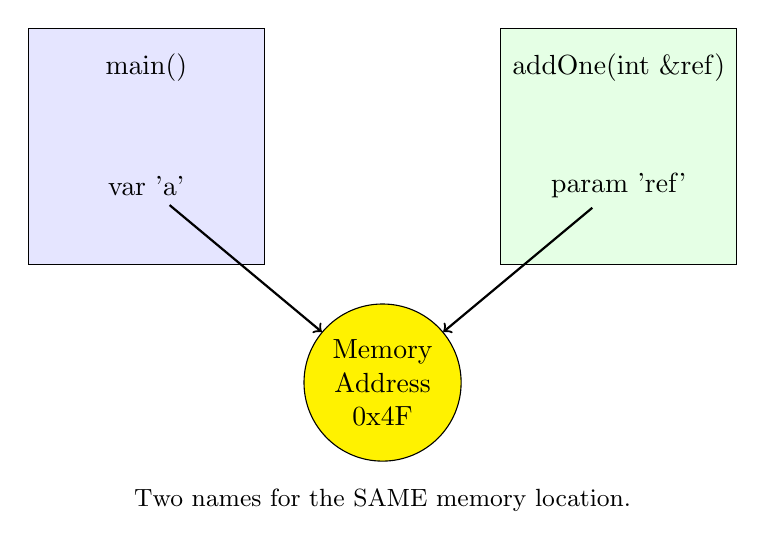
\begin{tikzpicture}
    % Main Scope
    \draw[fill=blue!10] (0,0) rectangle (3,3);
    \node at (1.5,2.5) {main()};
    \node (labelMain) at (1.5,1) {var 'a'};

    % Function Scope
    \draw[fill=green!10] (6,0) rectangle (9,3);
    \node at (7.5,2.5) {addOne(int \&ref)};
    \node (labelFunc) at (7.5,1) {param 'ref'};

    % Shared Memory
    \node[draw, fill=yellow, circle, minimum size=1.5cm, align=center] (mem) at (4.5, -1.5) {Memory\\Address\\0x4F};
    
    % Arrows
    \draw[->, thick] (labelMain) -- (mem);
    \draw[->, thick] (labelFunc) -- (mem);
    
    \node[align=center, font=\small] at (4.5, -3) {Two names for the SAME memory location.};
\end{tikzpicture}
\end{center}
\end{frame}

\begin{frame}[fragile]
\frametitle{Exercise 3: True Modification}
\textbf{Exercise File:} \texttt{scope\_04.cpp}

\pause
\textbf{Objective:} Use pass-by-reference to modify the original variable.

\pause
\begin{minted}[fontsize=\scriptsize, frame=lines, linenos]{cpp}
#include <iostream>
using namespace std;

// TODO 1: Change parameter to use '&' (int &val)
void trueModifier(int val) {
    val = val + 100;
    cout << "Inside: " << val << endl;
}

int main() {
    int x = 50;
    cout << "Before: " << x << endl;

    trueModifier(x);

    // TODO 2: Confirm x is now 150, not 50
    cout << "After: " << x << endl;
    return 0;
}
\end{minted}
\end{frame}

% ==========================================
% SECTION 5: SHADOWING
% ==========================================

\begin{frame}
\frametitle{Variable Shadowing}
\textbf{Shadowing} occurs when a variable in an inner scope has the same name as a variable in an outer scope.

\pause
\vspace{1em}
\begin{itemize}
    \item The \textbf{innermost} definition wins.
    \pause
    \item The outer variable is temporarily ``hidden'' or shadowed.
    \pause
    \item This creates confusion and should be avoided in production code.
\end{itemize}
\end{frame}

\begin{frame}[fragile]
\frametitle{Shadowing Puzzle}
\textbf{Predict the output:}

\pause
\begin{minted}[fontsize=\small]{cpp}
int x = 100; // Global

int main() {
    int x = 50; // Shadows Global

    if (x > 0) {
        int x = 10; // Shadows main's x
        cout << x << endl; // Prints 10
    }

    cout << x << endl; // Prints 50
    return 0;
}
\end{minted}
\end{frame}

% ==========================================
% SUMMARY
% ==========================================

\begin{frame}
\frametitle{Lesson Summary}
\begin{itemize}
    \item \textbf{Scope}: Where a variable lives.
    \pause
    \item \textbf{Local Variables}: Only exist inside their specific function (Safe).
    \pause
    \item \textbf{Global Variables}: Accessible everywhere (Unsafe/Messy).
    \pause
    \item \textbf{Pass by Value}: Functions get a \textbf{copy}. Original is safe. (Default for primitives).
    \pause
    \item \textbf{Pass by Reference}: Functions get an \textbf{alias} via \texttt{\&}. Original changes.
\end{itemize}

\pause
\vspace{1em}
\textbf{Rule of Thumb:} Always prefer local variables and pass them as parameters. Use references only when you intend to modify the data.
\end{frame}

\end{document}